\documentclass[10pt]{article}
\usepackage{mathtools}
\usepackage{amsmath}
\usepackage{tabularx}
\usepackage{graphicx}
\usepackage{flexisym}
\usepackage{listings}
\usepackage{xcolor}
\usepackage{hyperref}

\begin{document}
\setlength\parindent{1pt}
\title{Project 2}
\author{Andrei Kukharenka and Anna Gribkovskaya \\  
FYS 4150 
}

\maketitle
\begin{abstract}
In this work we solve the ... by .... .
\end{abstract}
\clearpage 


\section{Introduction}
\newpage
\section{Results and discussion}

\begin{table}
  \caption{One electron Jacobi.}
  \label{tab:one}
  \begin{center}
    \begin{tabular}{c|c|c|c|c}
    \hline
		$N$ & $Number of rotations$ & $\lambda_1$ & $\lambda_2$ & $\lambda_3$ \\
        \hline
	$	50 $  & $ 4036  $ & $2.77921$ & $6.65469$ & $10.5485$ \\
	$	100$  & $ 16521 $ & $2.88836$ & $6.82895$ & $10.7813$ \\
	$	200$  & $ 66745 $ & $2.94388$ & $6.91491$ & $10.8925$ \\
	$	300$  & $ 150755$ & $2.96252$ & $6.94338$ & $10.9288$ \\
	$	400$  & $ 269516$ & $2.97186$ & $6.95757$ & $10.9468$ \\

	\end{tabular}
  \end{center}
\end{table}

\begin{table}
  \caption{Two electrons Jacobi. N=200}
  \label{tab:two}
	\begin{center}
    \begin{tabular}{c|c|c|c|c}
    \hline
		$\omega$ & $Number\ of\ rotations$ & $\lambda_1$ & $\lambda_2$ & $\lambda_3$ \\
        \hline
		$0.01$ & $59717$ & $0.105776$ & $0.141516$  & $0.178049$ \\ 
		$0.5$  & $64207$ & $2.25271 $ & $4.17817 $  & $6.13601$ \\ 
		$1  $  & $64662$ & $4.11774 $ & $8.01741 $  & $11.966$ \\
		$5  $  & $66625$ & $17.8299 $ & $37.6929 $  & $57.7022$ \\

	\end{tabular}
  \end{center}
\end{table}


\begin{figure}
  \begin{center}
    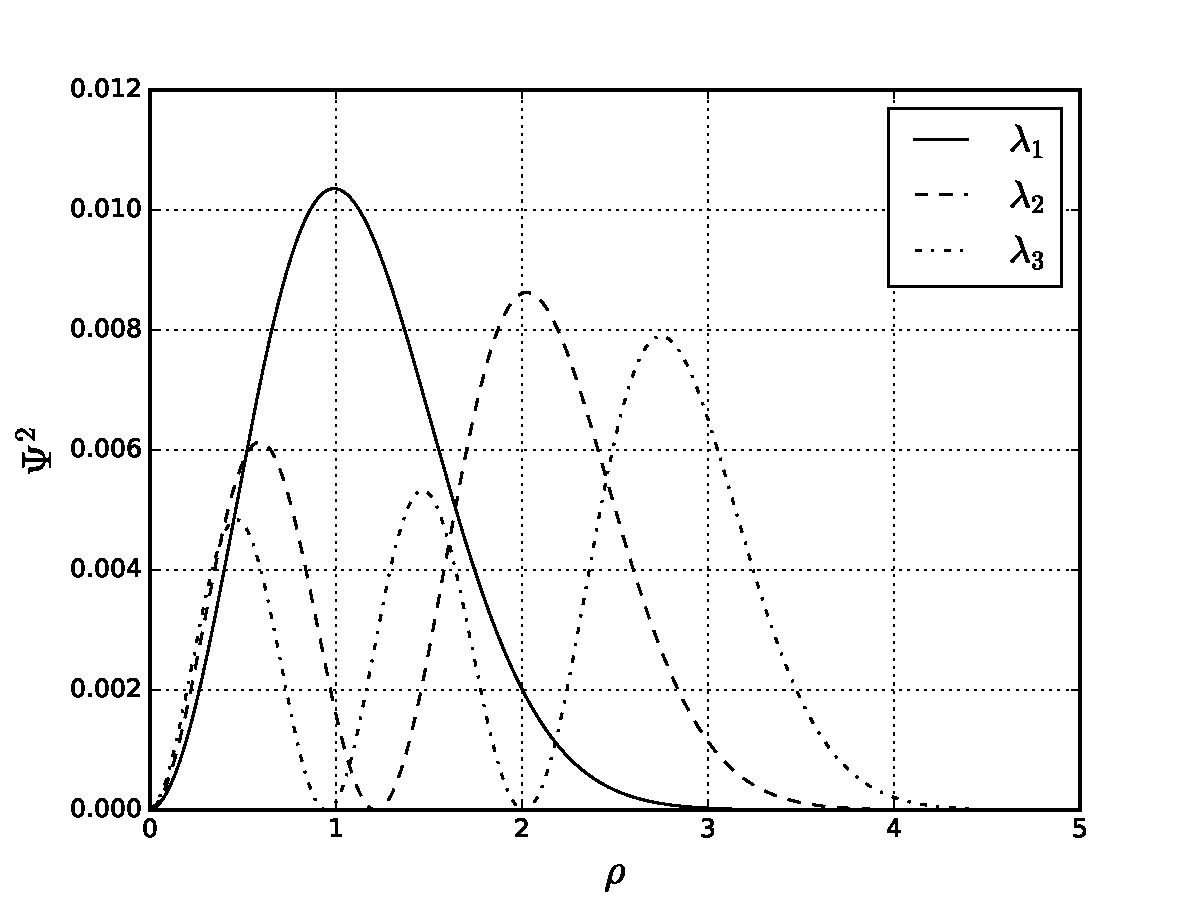
\includegraphics[scale=0.7]{one_electron}
    \caption{One electron}
    \label{fig:one_electron}
  \end{center}
\end{figure}

\begin{figure}
  \begin{center}
    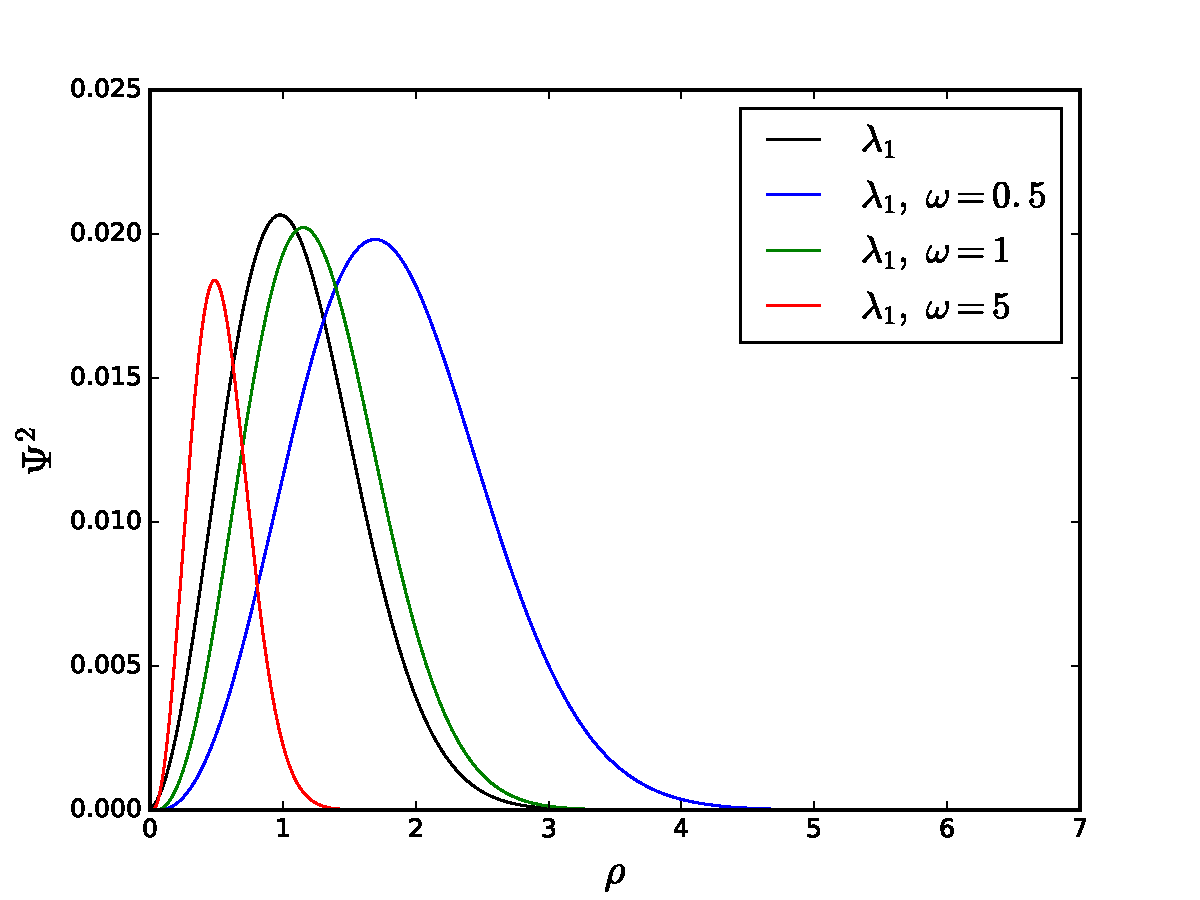
\includegraphics[scale=0.7]{compare}
    \caption{compare}
    \label{fig:compare}
  \end{center}
\end{figure}
\newpage
\begin{figure}
  \begin{center}
    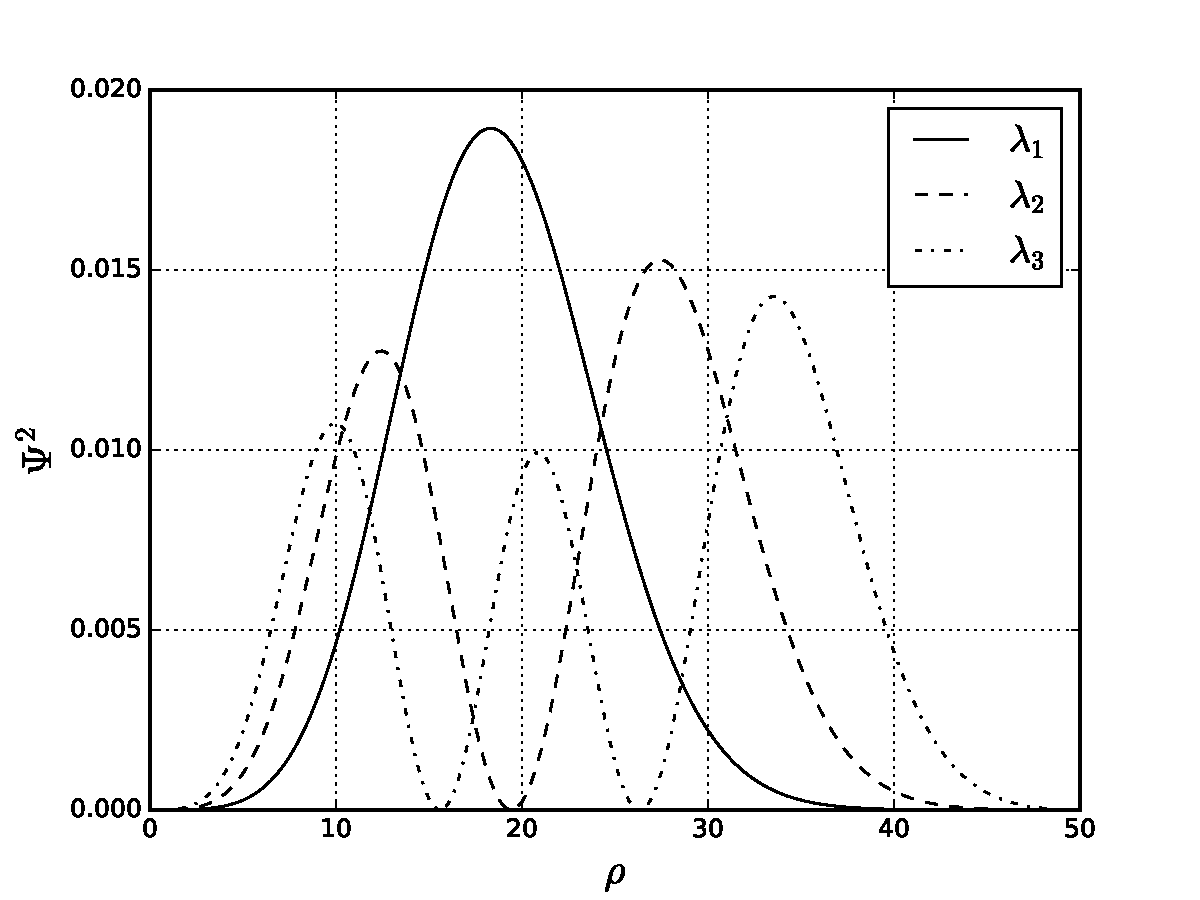
\includegraphics[scale=0.7]{two_001}
    \caption{0.01}
    \label{fig:omega_0.01}
  \end{center}
\end{figure}
\newpage

\begin{figure}
  \begin{center}
    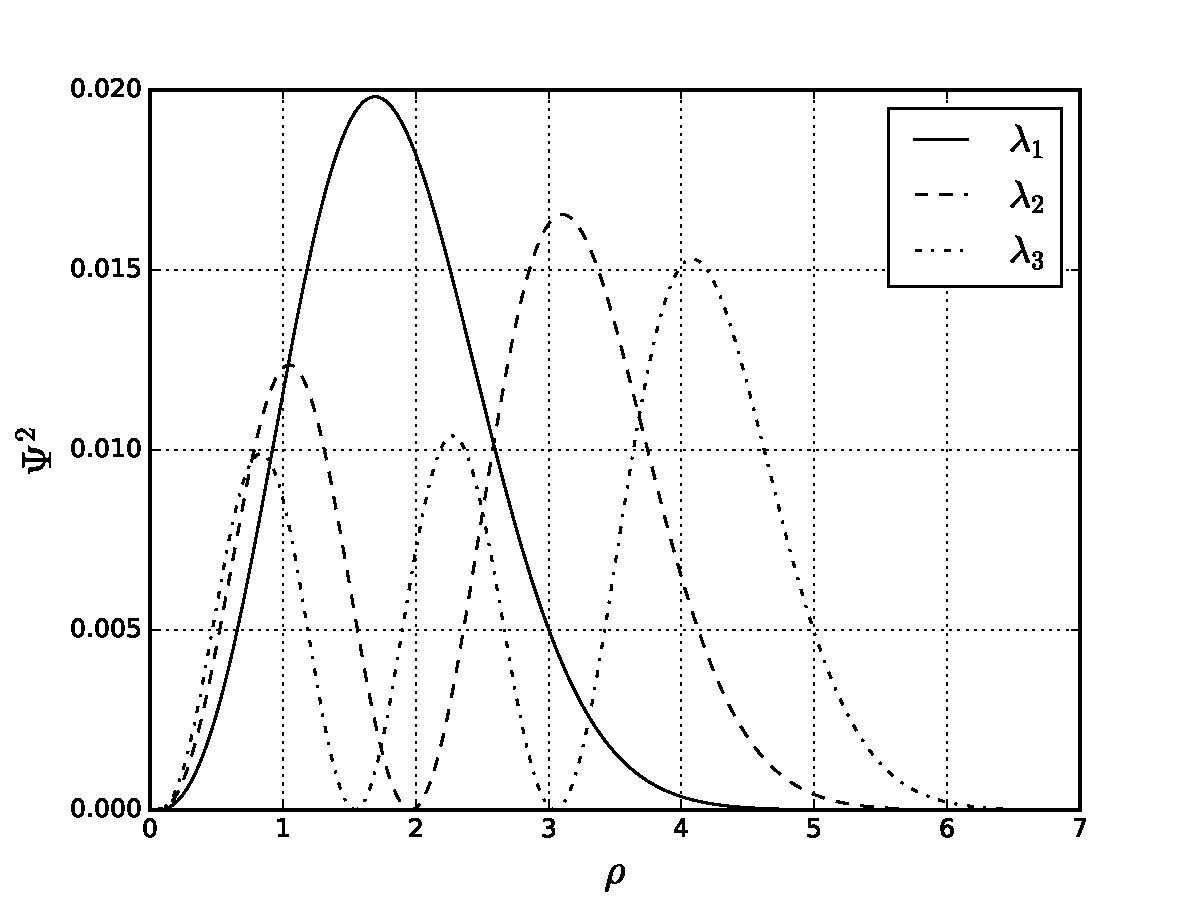
\includegraphics[scale=0.7]{two_05}
    \caption{0.5}
    \label{fig:omega_0.5}
  \end{center}
\end{figure}
\newpage

\begin{figure}
  \begin{center}
    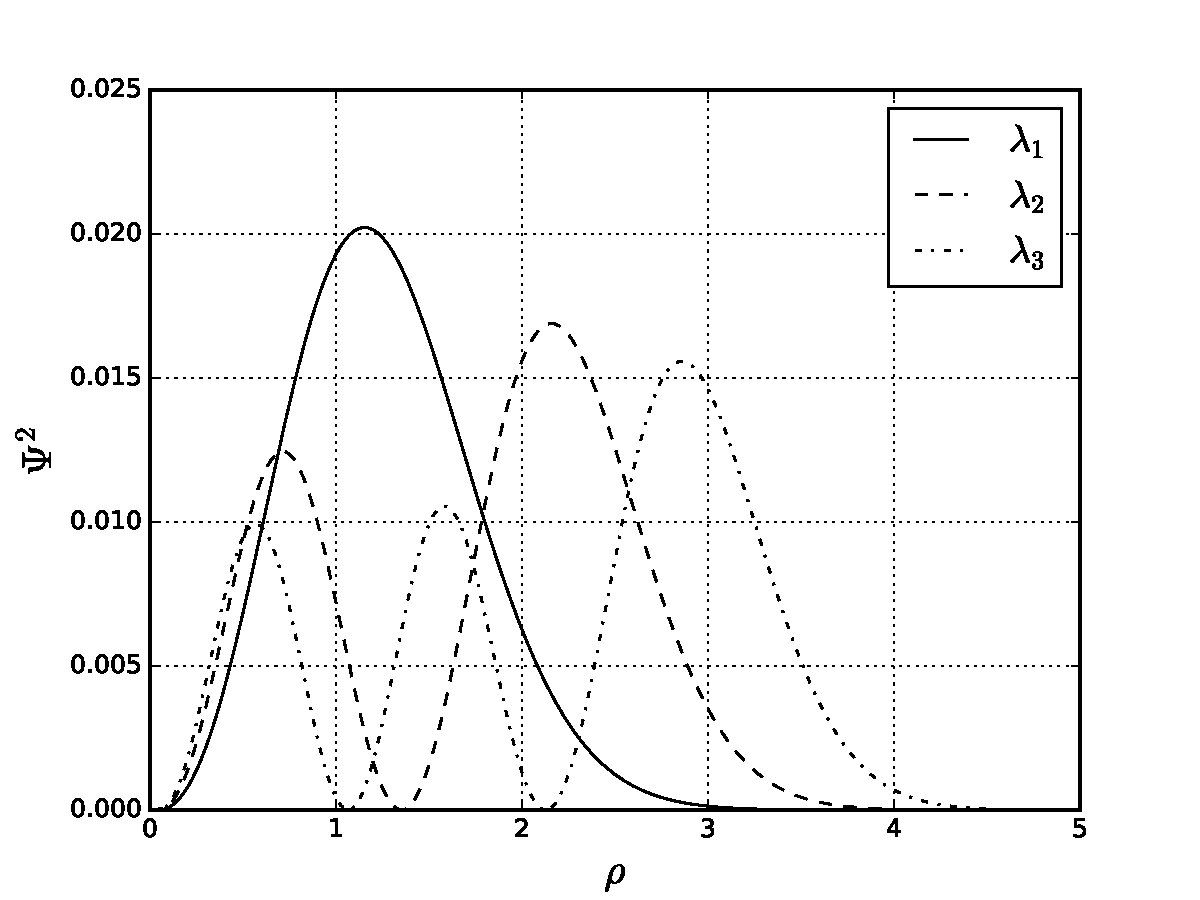
\includegraphics[scale=0.7]{two_1}
    \caption{1}
    \label{fig:omega_1}
  \end{center}
\end{figure}
\newpage

\begin{figure}
  \begin{center}
    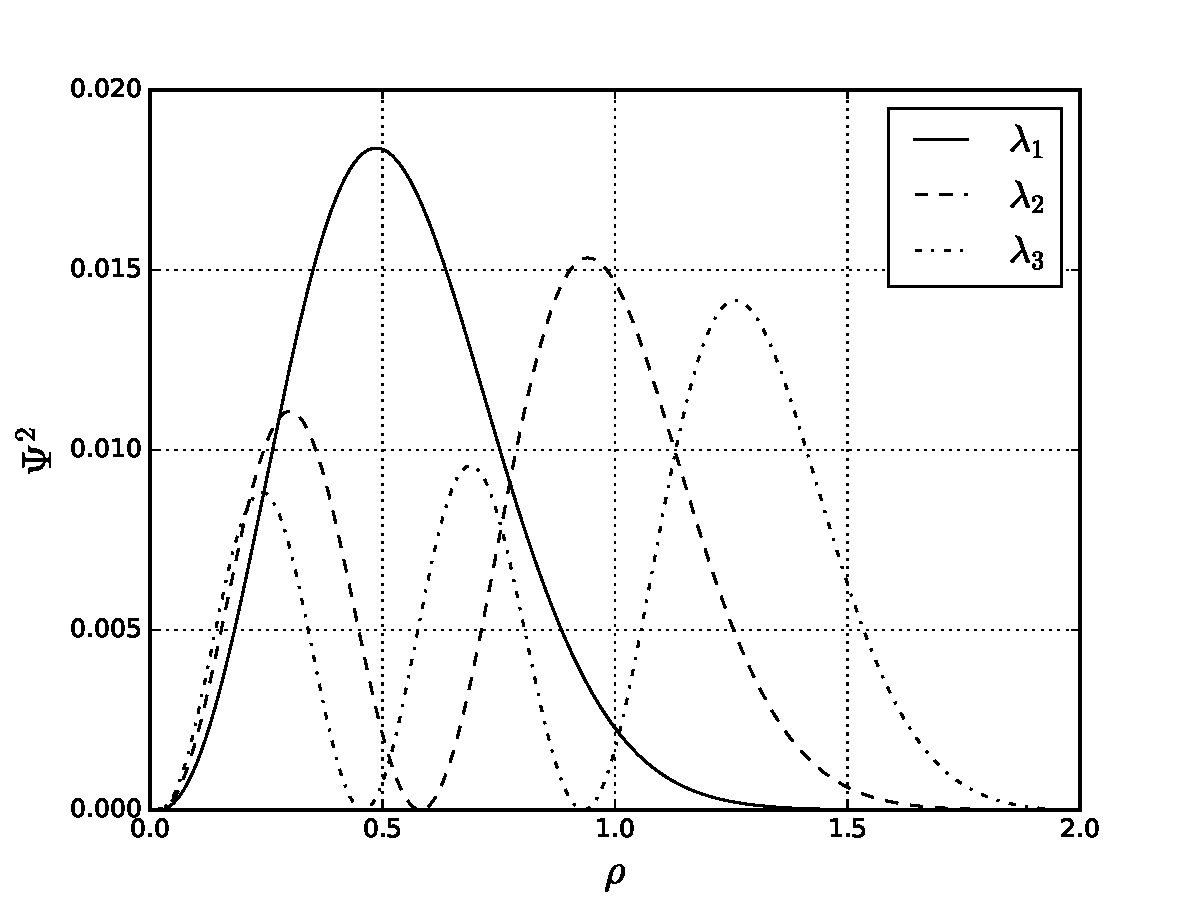
\includegraphics[scale=0.7]{two_5}
    \caption{5}
    \label{fig:omega_5}
  \end{center}
\end{figure}
\newpage


\section{Conclusion and further research}

\newpage
\begin{thebibliography}{2}
\bibitem{one} 
Morten Hjorth-Jensen. 
\textit{Computational Physics
}. 
Lecture Notes Fall 2015, August 2015.
 W. Press, B. Flannery, S. Teukolsky, W. Vetterling, Numerical Recipes in C++, The art of scientific Computing (Cambridge University Press, 1999)

\bibitem{two} 
W. Press, B. Flannery, S. Teukolsky, W. Vetterling 
\textit{Numerical Recipes in C++, The art of scientific Computing}. 
Cambridge University Press, 1999.
 
\end{thebibliography}

\end{document}
